\chapter{Event Reconstruction
\label{ch:reconstruction}}

Particles created in proton-proton collisions pass through the CMS detector and leave signals in different subdetectors. Figure \ref{fig:cms-slice} shows examples of typical signals for different types of particles. Each type of particle has a different characteristic signature from which it can be identified using information from the various subdetectors. Muons, electrons, and charged hadrons create tracks in the tracker, while photons and neutral hadrons do not. Muons also create hits in the muon systems. Electrons and photons deposit energy in the ECAL, while charged and neutral hadrons deposit most of their energy in the HCAL.

\begin{figure}[hbt]
\begin{center}
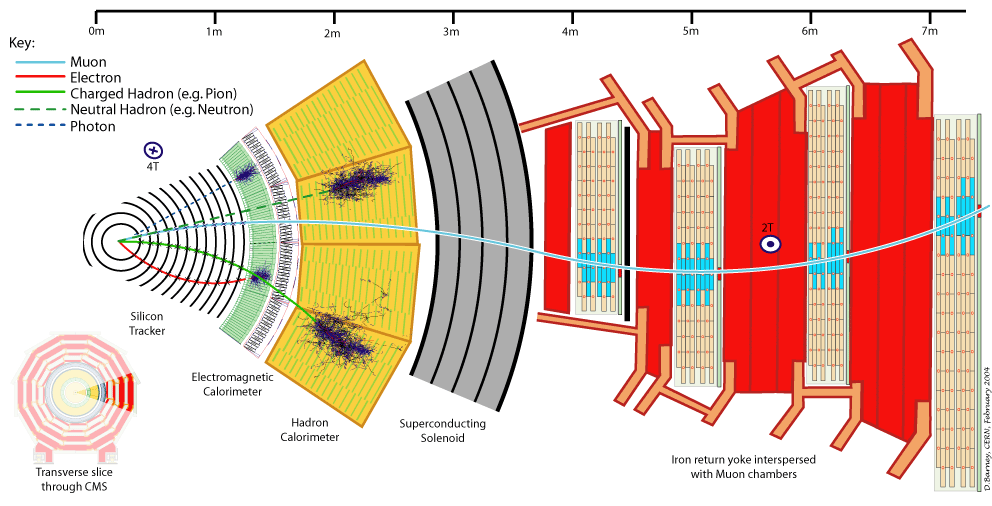
\includegraphics[width=0.95\textwidth]{figures/CMS_slice.png}
\caption{A cross-sectional view of the CMS detector with all subdetectors labeled and examples of signals left by muons, electrons, charged hadrons, neutral hadrons, and photons \cite{CMS-slice}.}
\label{fig:cms-slice}
\end{center}
\end{figure}

The raw output from each subdetector is processed in several steps in order to reconstruct the different types of particles \cite{TDR-software}. The first step is local reconstruction, which involves the creation of reconstructed hits or ``RecHits'' for each subsystem of each subdetector. The tracker RecHits include information about the positions of signals in the form of clusters, which are combinations of contiguous strips or pixels. The muon system RecHits also provide the positions of signals. In the DT and CSC subsystems, these RecHits can be combined into three-dimensional track segments. The ECAL and HCAL RecHits contain the energy, position, and time of energy deposits from traversing particles.

In the second step, global reconstruction, the RecHits from the different subsystems of a given subdetector are combined and further processed. In the tracker, pattern recognition algorithms are employed to reconstruct tracks for various cases, including displaced vertices, low \pt tracks, and high \pt tracks. The ECAL and HCAL RecHits are combined into calorimeter towers or ``CaloTowers'' using a projective $\eta$-$\phi$ geometry. ``Standalone'' muons are created by the muon system global reconstruction, which associates RecHits and track segments in a radial trajectory, accounting for bending by the residual magnetic field, and uses a vertex-constrained fit.

High-level reconstruction is the final step, in which information from all subdetectors is used to reconstruct various types of particles as precisely as possible. The particle types used in this search include electrons, muons, taus, jets, and b-jets. The reconstruction algorithms for these particles will be described in more detail in the following sections of this chapter. Many of these algorithms use a particle flow technique that is unique to CMS and will be described in Sec. \ref{sec:particle-flow}.

The CMS experiment uses detailed simulations to predict the performance of the detector and reconstruction algorithms and to model various physics processes. Each simulated event is generated from the interaction of partons in proton-proton collisions and the decays of the resulting particles, based on theoretical calculations. The traversal of the final state particles through the CMS detector is simulated to create simulated hits or ``SimHits''. The effects of photodetectors and readout electronics on these SimHits are also simulated. After that processing, the results can be treated identically to the raw data from real events and used as input for the reconstruction software.

\section{Event Generation}

\section{Detector Simulation}

\section{Tracks and Vertices
\label{sec:tracks}}

Hits from the different tracker subsystems are reconstructed into charged-particle tracks using the Combinatorial Track Finder (CTF) algorithm \cite{TrackingJINST}. CTF is an iterative algorithm which finds the easiest tracks first, in order to remove the associated hits from consideration. This reduces the complexity of finding more difficult tracks in subsequent iterations. Each iteration follows the same four-step procedure, varying the type of seed used and the selection criteria applied.
\begin{enumerate}
\item A seed is generated using only a few hits.
\item Additional hits are added to the track based on the extrapolated trajectory of the seed.
\item The parameters of the track are estimated using a fit which considers all hits in the trajectory.
\item Selection criteria are applied to determine the quality of the track, excluding those tracks which do not pass the selection.
\end{enumerate}

The types of seeds are categorized based on the number of hits included and the source of those hits. Initial iterations use pixel triplet and pair seeds, created from three and two pixel hits, respectively. These are the highest-quality seeds and are used to reconstruct prompt tracks, those emitting from primary vertices near the IP. A subsequent iteration uses a mixed triplet seed, containing 1--3 pixel hits and ${<}3$ strip hits. This iteration typically finds displaced tracks from heavy flavor decays, nuclear interactions, and photons which convert to \EpEm\xspace pairs in the tracker. The final iterations use strip pair seeds, consisting of two matched hits from the strip detectors, usually generated by charged particles which did not enter the pixel detector.

The iterations that use seeds with strip hits may also find prompt tracks which lack pixel hits. The specific sequence of iterations has been modified several times to improve the computing and physics performance of CMS tracking \cite{Tracking2012}. Table \ref{tab:tracking} lists the sequence used during the 2012 run. The selection criteria for each iteration are given, including cuts on \pt, transverse impact parameter $d_0$, and longitudinal impact parameter $z_0$. Some of the $z_0$ cuts are in terms of $\sigma$, the length of the beam spot in the $z$-direction used as a Gaussian standard deviation.

\begin{table}[htb]
  \begin{center}
    \begin{tabular}{llllll}
\hline
step  & seed type & seed subdetectors & \pt $[\GeVcns]$ & $d_0$ [cm] & $|z_0|$ \\
\hline
0     & triplet   & pixel             & ${>}0.6$     & ${<}0.02$  & ${<}4.0\sigma$ \\
1     & triplet   & pixel             & ${>}0.2$     & ${<}0.02$  & ${<}4.0\sigma$ \\
2     & pair      & pixel             & ${>}0.6$     & ${<}0.015$ & ${<}0.09\cm$ \\
3     & triplet   & pixel             & ${>}0.3$     & ${<}1.5$   & ${<}2.5\sigma$ \\
4     & triplet   & pixel/TIB/TID/TEC & ${>}0.5$--0.6 & ${<}1.5$   & ${<}10.0\cm$ \\
5     & pair      & TIB/TID/TEC       & ${>}0.6$     & ${<}2.0$   & ${<}10.0\cm$ \\
6     & pair      & TOB/TEC           & ${>}0.6$     & ${<}2.0$   & ${<}30.0\cm$ \\
\hline
    \end{tabular}
    \caption{The sequence of tracking iterations used during the 2012 run, including information on the seeds and selection criteria used in each step \cite{Tracking2012}.}
    \label{tab:tracking}
  \end{center}
\end{table}

The reconstructed tracks are used to reconstruct the primary vertices from the event \cite{TrackingJINST}. This includes both the main hard scatter vertex and additional vertices from pileup collisions. First, selection requirements are imposed on the tracks, in order to consider only prompt tracks near the IP. The selection requirements include cuts on the significance of $d_0$, the number of pixel and strip hits in the track, and the normalized $\chi^2$ from the fit of the track trajectory. The tracks which pass the selection requirements are clustered together using their $z$-coordinates, determined at each track's closest approach to the beam spot. A deterministic annealing algorithm is used to perform this clustering, in which each track may have a different probability to be associated with each vertex. The algorithm uses analogues of statistical mechanics quantities, slowly reducing the ``temperature'' and minimizing the ``free energy'' during each temperature iteration.

Once the deterministic annealing algorithm produces a list of vertex candidates, an adaptive vertex fitter is applied to each vertex candidate. This fitter weights each track in the vertex based on the agreement between the track and vertex positions. Using those weights, it fits the parameters of the vertex, including the $(x,y,z)$ position, the covariance matrix, and the number of degrees of freedom, $n_{\text{dof}} = -3 + 2 \sum{w_i}$, where $w_i$ is the weight for the $i$th track. The variable $n_{\text{dof}}$ can be used to select vertices which correspond to actual proton-proton interactions, as it is closely related to the number of tracks compatible with the vertex.

%add 2012 performance (efficiency, fake rate, vtx resolution)? references only have 2011 performance...

\section{Particle Flow
\label{sec:particle-flow}}

The CMS experiment uses a technique called particle flow (PF) to combine information from all subdetectors in order to identify all stable particles in each event \cite{CMS-PAS-PFT-09-001}. As described at the beginning of this chapter and shown in Fig. \ref{fig:cms-slice}, each type of stable particle is expected to create signals in a certain subset of the subdetectors. The performance of the PF algorithm was validated using early CMS data \cite{CMS-PAS-PFT-10-002,CMS-PAS-PFT-10-003}, along with newer CMS data for more recent uses of the algorithm \cite{Beaudette:2014cea}, demonstrating significant improvement over simpler approaches. The reconstructed particles are known as PF candidates, which can be treated as input particles by the various high-level reconstruction algorithms. PF candidates can also be used to compute the isolation of a reconstructed object, by summing the energy of candidates topologically close to the selected object.

The RecHits from the local reconstruction process are used to create the basic elements for this technique: tracks and clusters. Charged-particle tracks are created from tracker RecHits using an iterative algorithm as described in Sec. \ref{sec:tracks}, and muon tracks are created from muon system RecHits. Calorimeter energy deposits are grouped into clusters by identifying seed hits as local energy maxima exceeding a certain threshold, and then adding neighboring hits with energy above subsystem-specific thresholds meant to eliminate photodetector noise. Further removal of noise from the calorimeters is performed by rejecting clusters with characteristics matching those expected from leading sources of noise. Tracks and clusters are associated together using a linking algorithm that determines if they were likely produced by the same particle. The algorithm considers a possible link between each algorithm based on the $\eta$-$\phi$ distance between a charged-particle track and a cluster, or between two clusters. For links between a charged-particle track and a muon track, the $\chi^{2}$ value from a global fit is used as the link distance. Groups of elements are associated based on minimizing the link distance and are called ``blocks''.

PF reconstruction algorithms classify the blocks as different types of particles. When a block is classified as a certain type of particle, it is removed from the list of unclassified blocks. A global muon block is accepted as a PF muon if the momentum of the combined charged-particle and muon tracks agrees with the momentum of the charged-particle track alone. The energy expected to have been deposited by the PF muons in the calorimeters due to minimum ionization is subtracted from the clusters. The remaining charged-particle tracks are checked for compatibility with electrons, which tend to leave short tracks and radiate energy via bremsstrahlung. A Gaussian Sum Filter (GSF) is applied to the compatible tracks in order to identify spatially-matched ECAL clusters, and the combination of a track and one or more clusters is classified as a PF electron.

The remaining tracks are linked to clusters to form PF charged hadrons, if the total cluster energy is similar to but smaller than the total track momentum. More than one track can link to a given cluster, but for a given track, only the link to the closest cluster is kept. This reflects the coarser segmentation of the calorimeter system as compared to that of the tracker. In cases where the total cluster energy is significantly smaller than the total track momentum, additional PF muons may be found using tracks from the block, and some tracks may be classified as fake and removed from consideration. Finally, an excess of energy in the clusters, above the total track momentum, is assumed to come from neutral particles. The excess energy is typically classified as a PF photon. If the total excess cluster energy in a block is larger than the total ECAL energy in the cluster, a PF neutral hadron is created from the excess energy remaining after assigning the ECAL excess energy to a PF photon. The remaining clusters not linked to any tracks are used to create PF photons in ECAL and PF neutral hadrons in HCAL.

\section{Electrons}

\section{Muons}

\section{Taus}

\section{Jets}

\section{b-tagging}